\documentclass[10pt,twocolumn,letterpaper]{article}

\usepackage{cvpr}
\usepackage{times}
\usepackage{epsfig}
\usepackage{graphicx}
\usepackage{amsmath}
\usepackage{amssymb}
\usepackage{caption}
\usepackage{subcaption}

% Include other packages here, before hyperref.

% If you comment hyperref and then uncomment it, you should delete
% egpaper.aux before re-running latex.  (Or just hit 'q' on the first latex
% run, let it finish, and you should be clear).
\usepackage[breaklinks=true,bookmarks=false]{hyperref}

\cvprfinalcopy % *** Uncomment this line for the final submission

\def\cvprPaperID{****} % *** Enter the CVPR Paper ID here
\def\httilde{\mbox{\tt\raisebox{-.5ex}{\symbol{126}}}}

% Pages are numbered in submission mode, and unnumbered in camera-ready
%\ifcvprfinal\pagestyle{empty}\fi
\setcounter{page}{1}
\begin{document}

%%%%%%%%% TITLE
\title{Two Class Semantic Segmentation Applied to Autonomous Vehicle Road Detection}

\author{Dwight Brisbin\\
University of Michigan\\
500 S State St. Ann Arbor MI, 48109\\
{\tt\small dbrisbin@umich.edu}
}

\maketitle
%\thispagestyle{empty}

%%%%%%%%% ABSTRACT
\begin{abstract}
   The problem of distinguishing the road from the rest of the environment is a critical component of any competent autonomous driving system. This task has been largely solved in recent years by using an encoder-decoder network architecture. Many of these networks are purpose built for this task, but it would be interesting to see how a general purpose segmentation network performs for road segmentation. This paper discusses the problem of road segmentation and achieves high accuracy using four different general purpose segmentation architectures.
\end{abstract}

%%%%%%%%% BODY TEXT
\section{Introduction}
One of the key components of a robust autonomous vehicle system is highly accurate road and lane detection. A common approach is to apply semantic segmentation. Semantic segmentation is a process where elements or regions in the environment are classified according to a set of semantic labels. In addition to autonomous driving, this widely applicable technique has been used in robotics, interactive systems, medical imaging, and creative applications. In the past decade, methods to perform this task have all but completely solved the road segmentation problem, offering both real-time inference and very high accuracy. This paper introduces the major methods used over the last ten years to this challenge, including the primary datasets and architectures. Then, we will discuss in more depth the specific architectures chosen to perform testing on. Following, I will share experimental details and results. The paper will conclude with a discussion of this work. 

The code for this project can be found at \url{https://github.com/ddbrisbin/semantic-segmentation-pytorch}.

%------------------------------------------------------------------------
\section{Related Work}
As mentioned, the road segmentation problem is a simplification of the more general semantic segmentation problem. This section will discuss both of these problems including the common approaches and examplar projects. One of the key components of research in this area is good data. A number of useful datasets have been developed to solve the road segmentation problem which we also discuss here.

\begin{figure}[t]
\begin{center}
    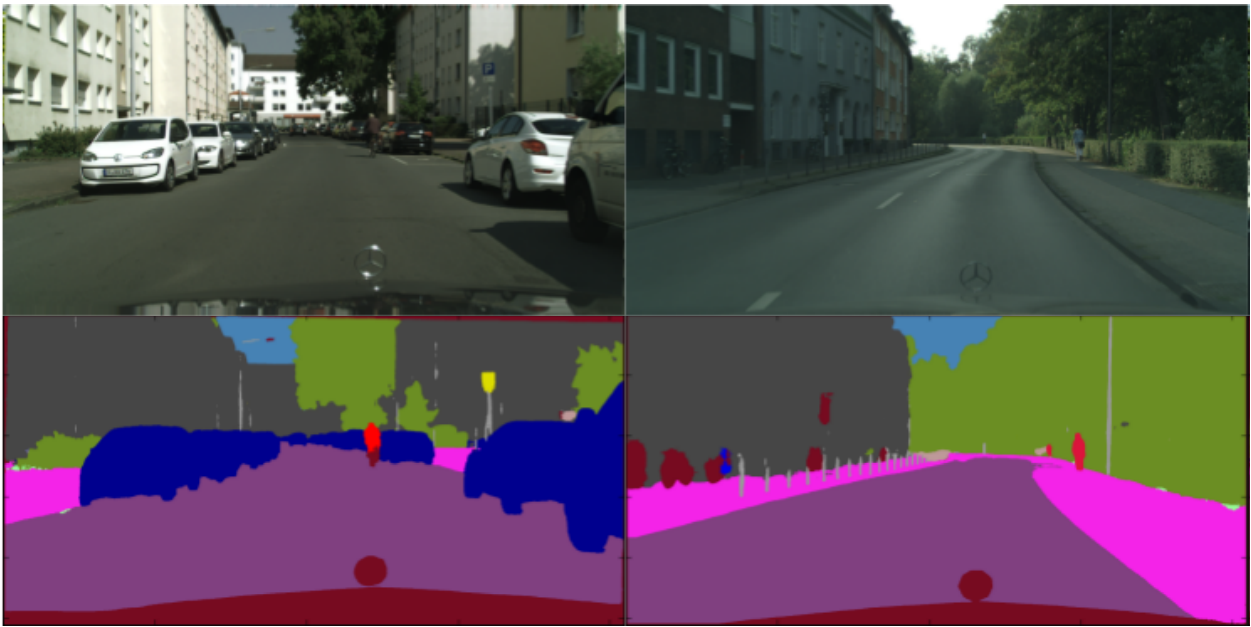
\includegraphics[width=\linewidth]{images/sampleseg.png}
\end{center}
   \caption{Two examples of semantic segmentation in autonomous vehicles. The top images are scenes from the Cityscapes dataset and the bottom images are semantic maps generated by the network described in \cite{Treml18}. Here, the segmentation is the same resolution as the original image, as in most segmentation networks for autonomous vehicles.}
\label{fig:sampleseg}
\end{figure}

\subsection{Segmentation for Autonomous Vehicles}
When applied to autonomous vehicles, we are most interested in constructing a semantic map of the same resolution of the original image, as in Figure \ref{fig:sampleseg}
The majority of successful architectures for semantic segmentation in autonomous vehicle perception follow an encoder-decoder architecture. In the encoder portion, successful classification networks are often used, that is, networks which accurately classify the \textit{presence} of a class-member, agnostic of spatial information. One key issue that arises; however, is that useful spatial information cannot be recovered from the downsampled result of the encoder since we need to match the original resolution. The solution is to use an decoder to upsample the image to the original resolution, extracting the spatial segmentation throughout these layers. The decoder used is almost always learned as opposed to traditional image upsampling techniques. Another technique used to improve performance are skip connections, which are used between the layers of the encoder and decoder with the same resolution to combine the original predictions from the encoder side with the decoder.

\begin{figure}[t]
\begin{center}
    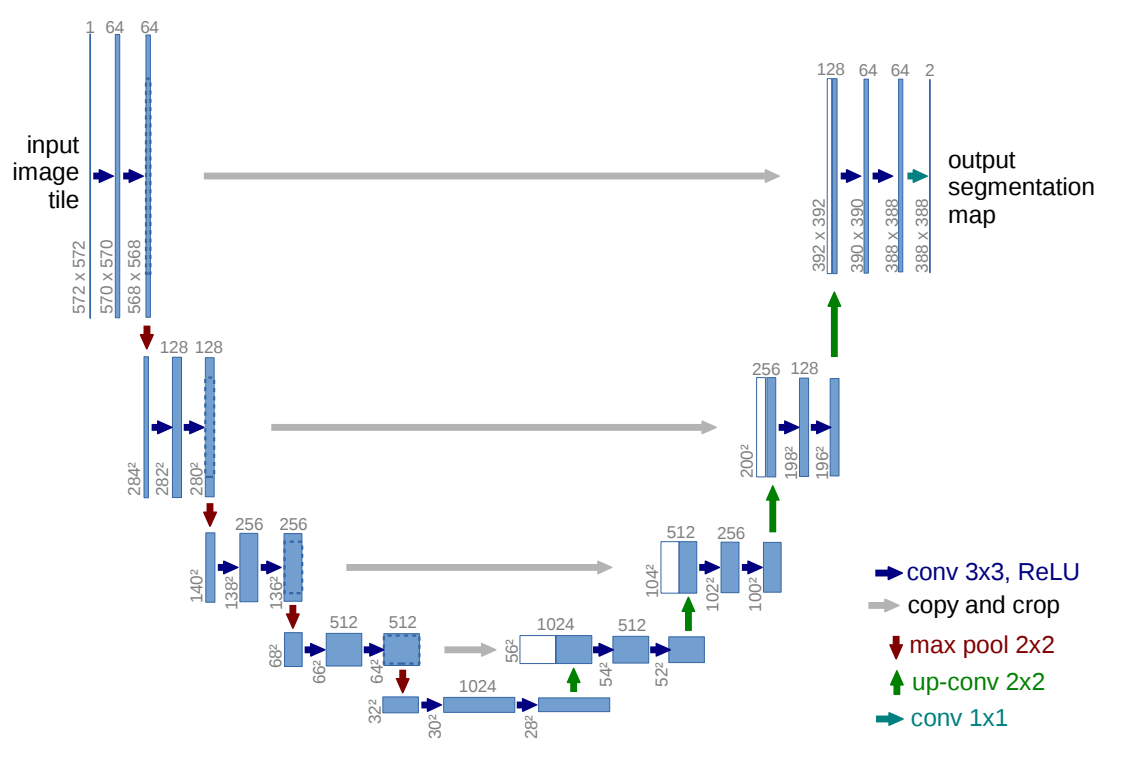
\includegraphics[width=\linewidth]{images/unet_arch.PNG}
\end{center}
   \caption{The U-net architecture for an input image resolution of 572 $\times$ 572. The numbers to the lower left of the layers represent the size and the numbers above represent the number of channels. The gray arrows here are skip connections.}
\label{fig:unet}
\end{figure}

One of the first very successful approaches using all of the above ideas was U-Net \cite{Ronneberger_2015}. Its architecture is shown in Figure \ref{fig:unet}. This network was originally applied to segmentation for images in the biomedical field, but has had tremendous influence across many other fields, with over 13,000 citations. More advanced variants of this architecture have since had tremendous success in road segmentation for autonomous vehicles. The network does not employ any expensive fully connected layers and the skip connections allow for fewer parameters as they propagate useful information directly. Both of these design choices lend to a network which was faster than many of its predecessors. It is this architecture which inspired a great deal of follow-on work, which in the autonomous vehicle space gave way to real-time, high-accuracy networks with rapid training.

The architecture and a good backbone encoder are the primary components required for fast and accurate performance on the road segmentation task, but there are a few other important techniques which papers in this space often employ. First, many papers use pretrained weights for the encoder as a starting point which allows for faster convergence. Second, many follow-on architectures of U-net have employed skip connections \textit{within} the encoder or decoder, in addition to \textit{between} the encoder and decoder. This is another technique which provides quicker convergence and it also allows for deeper networks to be trained. A final technique is to swap some pooling layers with dilated convolution layers which more accurately retain spatial details.

Overall, a great many networks have been developed to solve this problem with great success. In my experiments, I look at several combinations of different encoders and decoders, guided by work out of MIT's CSAIL I will discuss these in greater detail in section 3.

\subsection{Datasets for AV Segmentation}
Large and varied datasets are of critical importance to research in developing new networks for road segmentation. Over the last several years the amount of available annotated data for this task has increased dramatically. Let us look at some of the more common ones briefly:

\begin{itemize}
    \item KITTI: The KITTI road segmentation dataset is one of the older available datasets and has very rich data including LiDAR measurements, stereo camera images, GPS and IMU measurements and grayscale camera images. This dataset has a wide variety of scenes in its less than 300 images, which is useful for testing how a system could perform with little training data. This is the dataset my experiments use.\cite{Fritsch13}
    \item BDD100K: This is a relatively new dataset out of Berkeley and it is by far the largest publicly available dataset. This dataset has about 120 million images across 100,000 driving sequences in several driving conditions. \cite{yu18}
    \item Cityscapes: This is another popular, standard semantic segmentation dataset for self-driving cars somewhat similar to KITTI, but it places an emphasis on urban scenes. It only consists of approximately 5,000 finely annotated images and an additional 20,000 weakly annotated. \cite{Cordts16}
    \item Mapillary Vistas: This is a moderately sized dataset with 25,000 high-quality images fully annotated. This dataset also includes multiple viewpoints (for example, from a sidewalk) that you do not get from a car. This is not especially useful data for the defined problem, but there are extensions which would be assisted by having extra viewpoints. This dataset includes data from 5 different continents. \cite{Neuhold17} 
\end{itemize}

There are many other popular datasets, and the above are just a small sample of what is available.
\begin{figure*}[h]
\begin{center}
    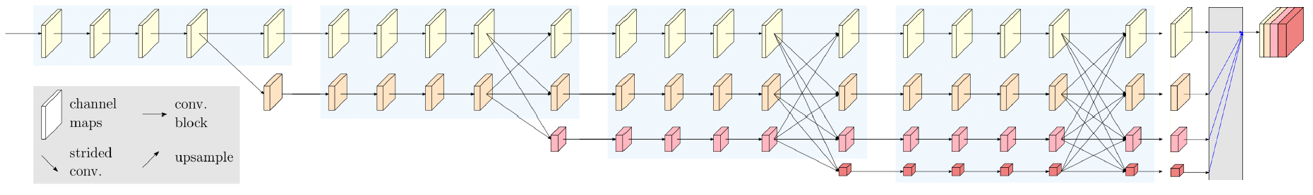
\includegraphics[width=\linewidth]{images/seg-hrnet.png}
\end{center}
   \caption{The HRNetV2 architecture. The key element of this architecture (in contrast to U-Net shown above) is that the resolution is carried through the entire network.}
\label{fig:hrnet}
\end{figure*}

\begin{figure*}[h]
\begin{center}
    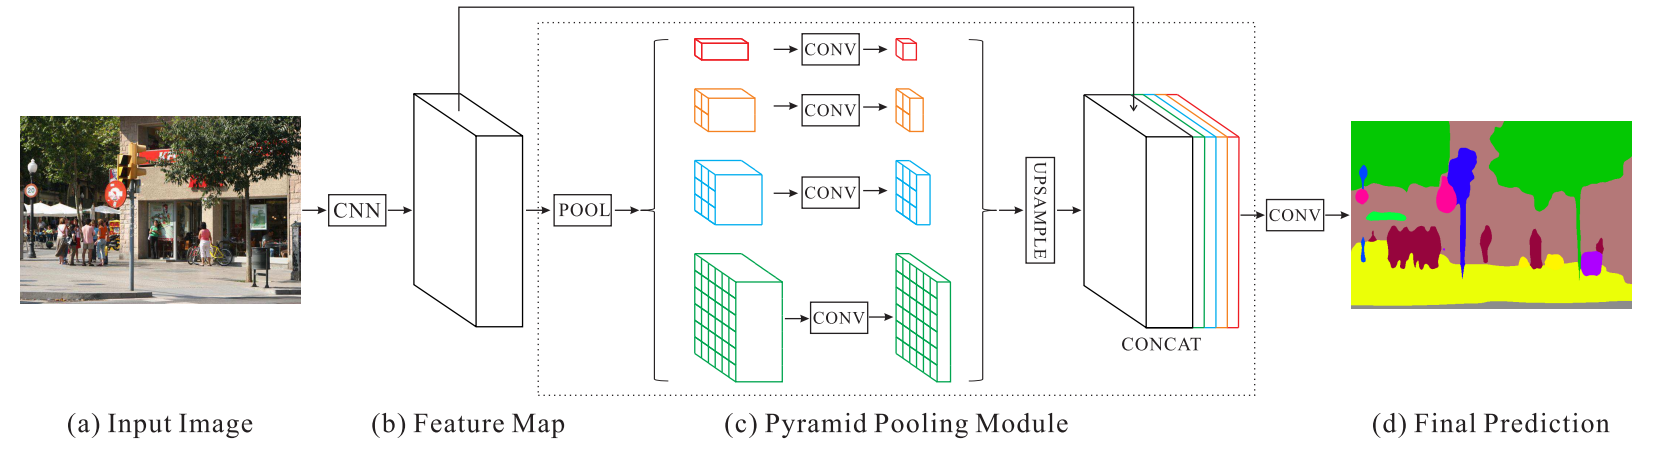
\includegraphics[width=\linewidth]{images/PSP.png}
\end{center}
   \caption{Pyramid Scene Parsing Network using the pyramid pooling module.\cite{Zhao17}}
\label{fig:PSP}
\end{figure*}

\section{Method}
For my exploration of this problem, I wanted to see how well high-performing, general purpose networks could do for road detection with limited data. To that end, I selected the MIT CSAIL Vision semantic segmentation project to use in my experiments. This project implements five different encoders and five different decoders (total number of possible combinations is 25) and applies them to the MIT ADE20K dataset \cite{zhou18}. This dataset consist of far more images than the KITTI dataset I worked with and accomodates many more classes than the two I am working with. Still, the networks they use have proven very successful for general segmentation problems.

\subsection{Encoders}
The first component in most road segmentation networks is the encoder, which is discussed in a previous section. The MIT project implements three major classes of network for the encoder, with three variants of ResNet for a total of five. 
\subsubsection{HRNet}
The first encoder I used is HRNet. This approach was fairly original when it came out because the trend had been towards faster networks by reducing resolution and subsequently upscaling. HRNet instead carries the original resolution throughout the process in addition to downscaled versions and reconstructs them at the end. This approach should lead to results which are more precise because the original spatial information is always available. This network alone gave state of the art results on some of the major semantic segmentation datasets, including Cityscapes. A diagram of this networks architecture is shown in Figure \ref{fig:hrnet}.

\subsubsection{ResNet}
ResNet and its variants are some of the most important modern networks. The key idea is that we are interested in having very deep networks, but in doing so, the gradients become too small to perform any meaningful updates during training. The solution that ResNet introduced was to use an ``identity shortcut" which skips multiple layers. This approach allowed for extremely deep networks (the authors have shown that a network with a depth over 1000 is still an improvement over small networks) and the approach quickly caught on \cite{He16}. In my experiments, I use both the 101 and 50 variants of ResNet.

\subsubsection{MobileNet}
The class of networks called MobileNets were introduced in 2017 by Google. The motivation behind the architecture is to create very lightweight, deep networks. These networks have proven to have high performance across a wide variety of segmentation tasks. \cite{Howard17}.

\begin{figure*}
\centering
    \begin{tabular}{|l|l|c|c|c|}
        \hline Encoder Architecture & Decoder Architecture & Overall Accuracy & Road IoU & Environment IoU \\ \hline
        MobileNetV2-Dilated & Single convolution layer & 98.41\% & 0.9202 & 0.9805 \\
        HRNetV2 & Single convolution layer & 98.58\% & 0.9409 & 0.9202 \\
        ResNet101 & UPerNet & 97.92\% & 0.9416 & 0.9793 \\
        ResNet50-Dilated & Pyramid Pooling Module &\textbf{ 98.90}\% & \textbf{0.9435} & \textbf{0.9835} \\
        \hline
    \end{tabular}
\caption{The results from my experimentation. The encoder/decoder pair ResNet50-Dilated/Pyramid Pooling Module performed the best on every tracked metric.}
\label{fig:resultsTable}
\end{figure*}

\subsection{Decoders}
The MIT project implements three classes of algorithm for the decoder.

\subsubsection{Convolution}
The first implementation is just a single convolutional layer. In theory this should perform quite well with at least HRNet since that network already produces good estimates of semantic segmentation.

\subsubsection{Pyramid Pooling Module}
The Pyramid Pooling Module (PPM) is a component of PSPNet out of The Chinese University of Hong Kong \cite{Zhao17}. This approach fuses features out of a convolutional net under different scales. Each of these scales is put through a convolution and concatenated to give a final prediction. The architecture for this approach is shown in Figure \ref{fig:PSP}.

\subsubsection{UPerNet}
UPerNet was developed to approach the novel task of ``Unified Perceptual Parsing". This task attempts to solve several different vision tasks simultaneously including segmentation, detection, scene recognition, and texture identification \cite{Xiao18}.

\section{Experiments}
For my experiments, I wanted to see if modern general purpose segmentation algorithms could be readily applied to road segmentation. To that end, I chose to use the KITTI dataset discussed above because it has a very small size, meaning that I could compare several trained networks. In addition, using KITTI would test the hypothesis of whether small datasets are sufficient for robust road detection.

Given that my goal was to test several different networks, it was more practical to use an existing implementation of these. I chose the MIT CSAIL semantic segmentation repo because it offered several different networks with all of the utilities I needed. I originally intended to directly replicate results of existing novel approaches; however, I could not get any of the candidates running for a suitable baseline.

The major changes I had to make to the MIT implementation were constructing the correct files separating the training and validation images and creating configuration files for each of the tests I ran. I achieved the former by writing a MATLAB script to separate the images and annotations with an 80-20 training-validation ratio and construct the requisite files (included in the project repo). The latter was less straightforward as I had to reason about how to modify the hyperparameters for optimal performance with a significantly smaller dataset (221 images compared to 20,000). The configuration files for each experiment is included in the GitHub repo and is straightforward to read, so these are omitted from the writeup for brevity.

It took about 20 hours to train the four of the seven networks I had intended to test. Unfortunately, I did not have more time to train the rest and include in this report. I will now discuss the results of the experiment.

\subsection{Results}
I was quite pleased with the performance of each of the networks. I expected the HRNet encoder/convolution decoder to perform the best because HRNet is a very recent network known to perform quite well on semantic segmentation for urban driving. Since the road segmentation problem is a subset, I figured HRNet would still do quite well. In reality, the best performing network was ResNet50 paired with a pyramid pooling module, with an accuracy approaching 99\%. The full results are shown in Table \ref{fig:resultsTable}. I have also included images of the segmentations created by the networks in Figure \ref{fig:samples}.

\begin{figure*}
    \centering
    \begin{subfigure}[t]{\linewidth}
        \centering
        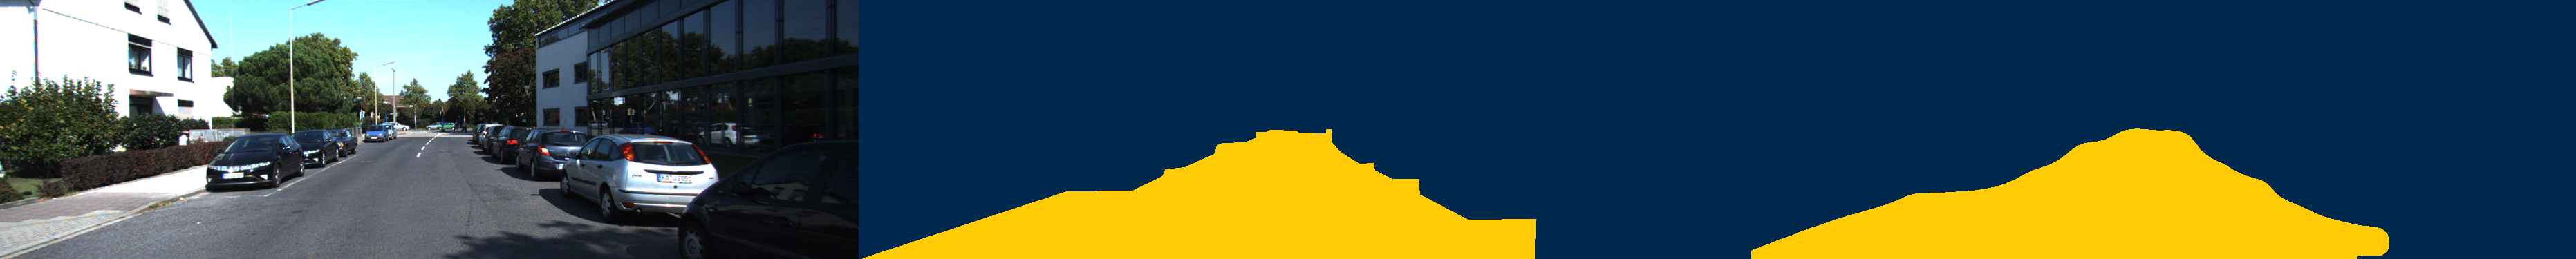
\includegraphics[width=0.9\linewidth]{images/mn_a.png}
        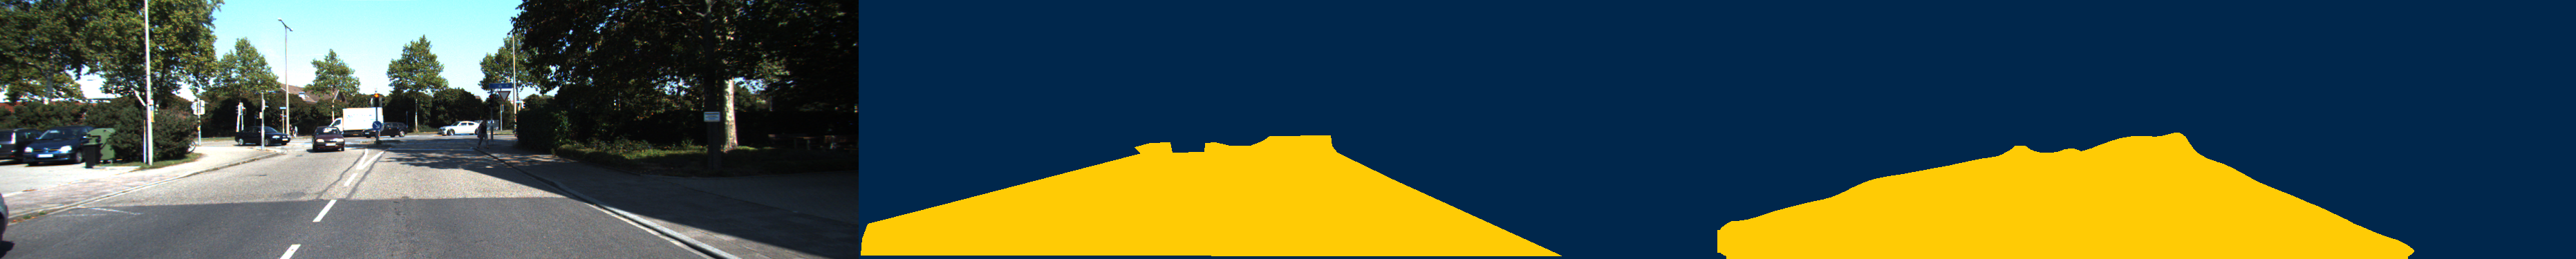
\includegraphics[width=0.9\linewidth]{images/mn_b.png}
        \caption{MobileNetV2-Dilated with Single convolution layer}
    \end{subfigure}
    \begin{subfigure}[t]{\linewidth}
        \centering
        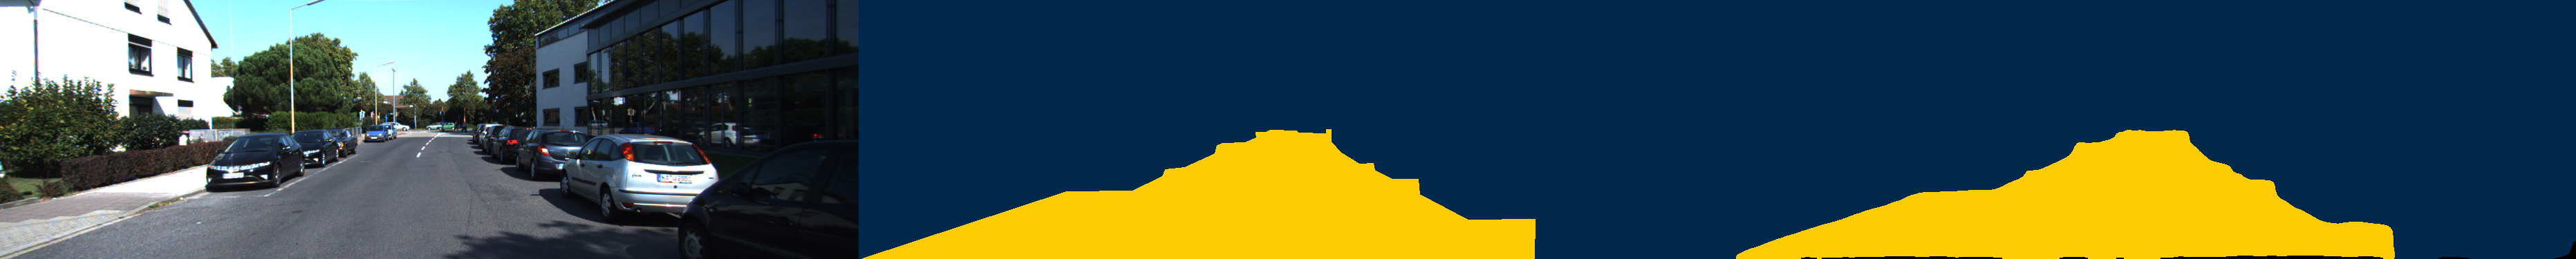
\includegraphics[width=0.9\linewidth]{images/hr_a.png}
        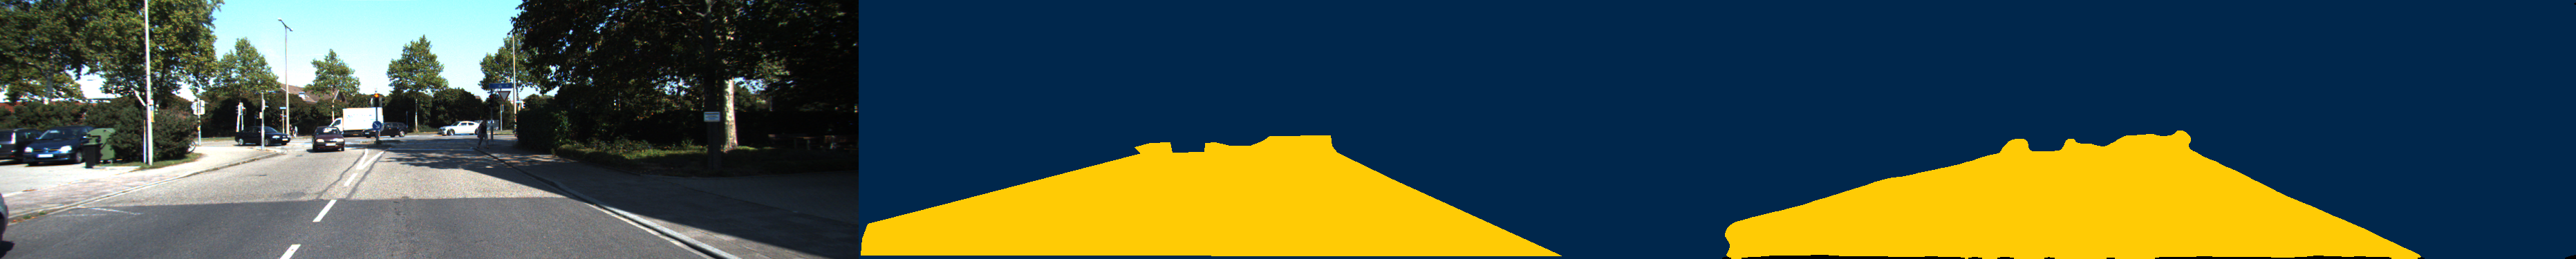
\includegraphics[width=0.9\linewidth]{images/hr_b.png}
        \caption{HRNetV2 with Single convolution layer}
    \end{subfigure}
    \begin{subfigure}[t]{\linewidth}
        \centering
        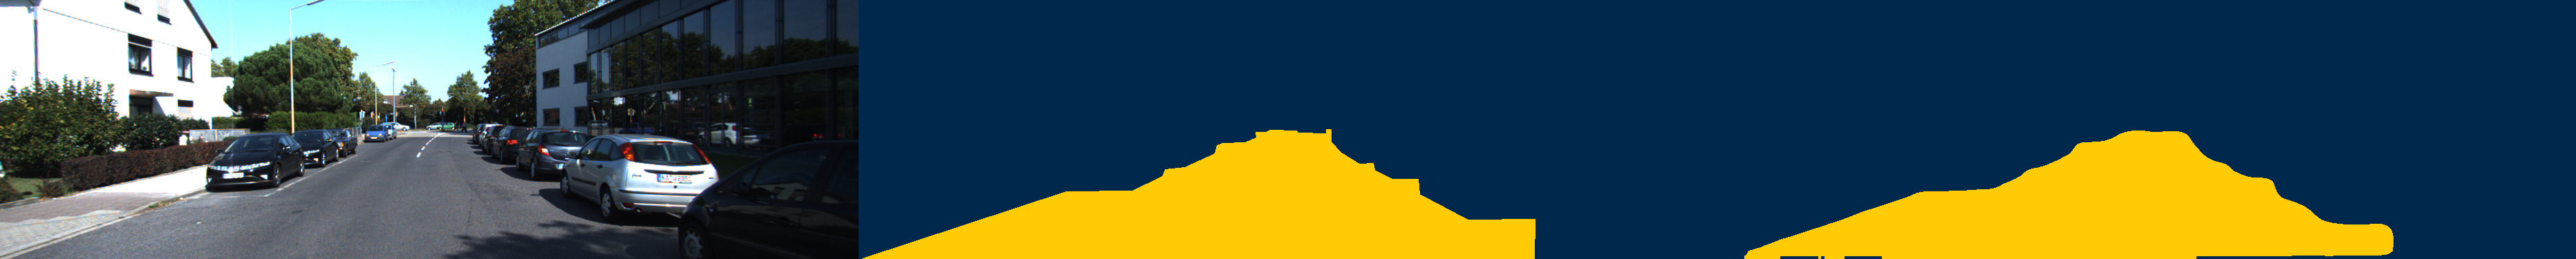
\includegraphics[width=0.9\linewidth]{images/rn50_a.png}
        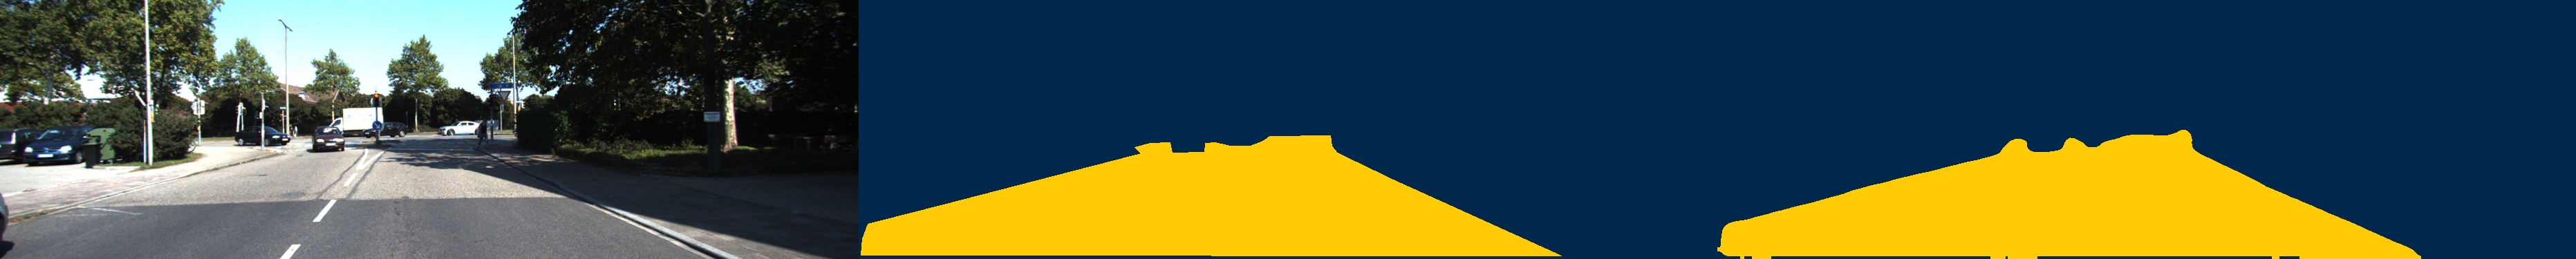
\includegraphics[width=0.9\linewidth]{images/rn50_b.png}
        \caption{ResNet101 with UPerNet}
    \end{subfigure}
    \begin{subfigure}[t]{\linewidth}
        \centering
        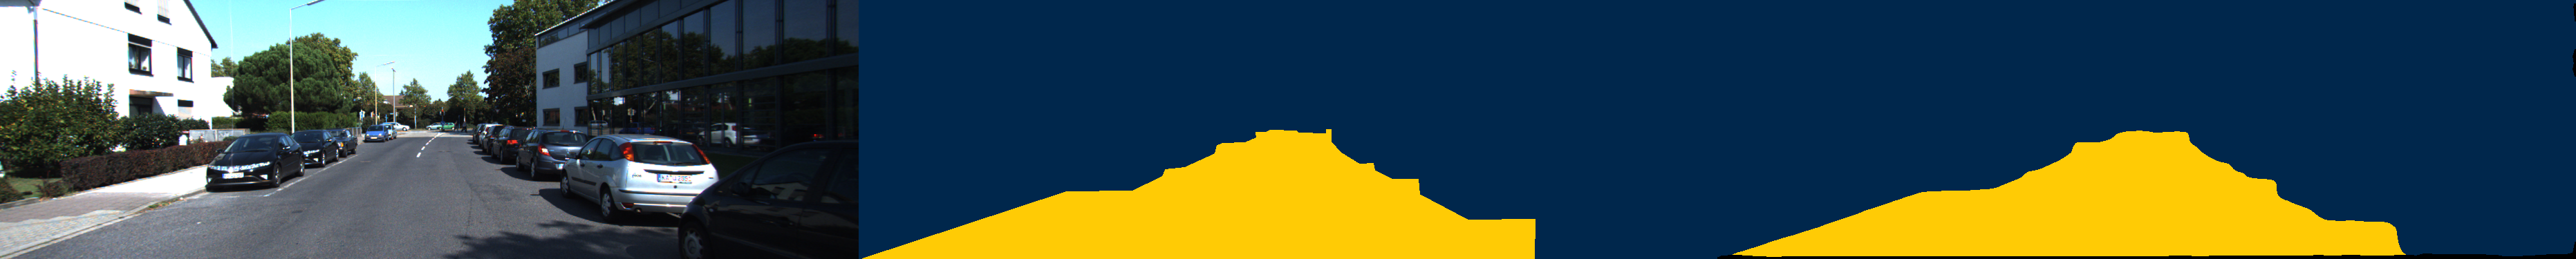
\includegraphics[width=0.9\linewidth]{images/rn100_a.png}
        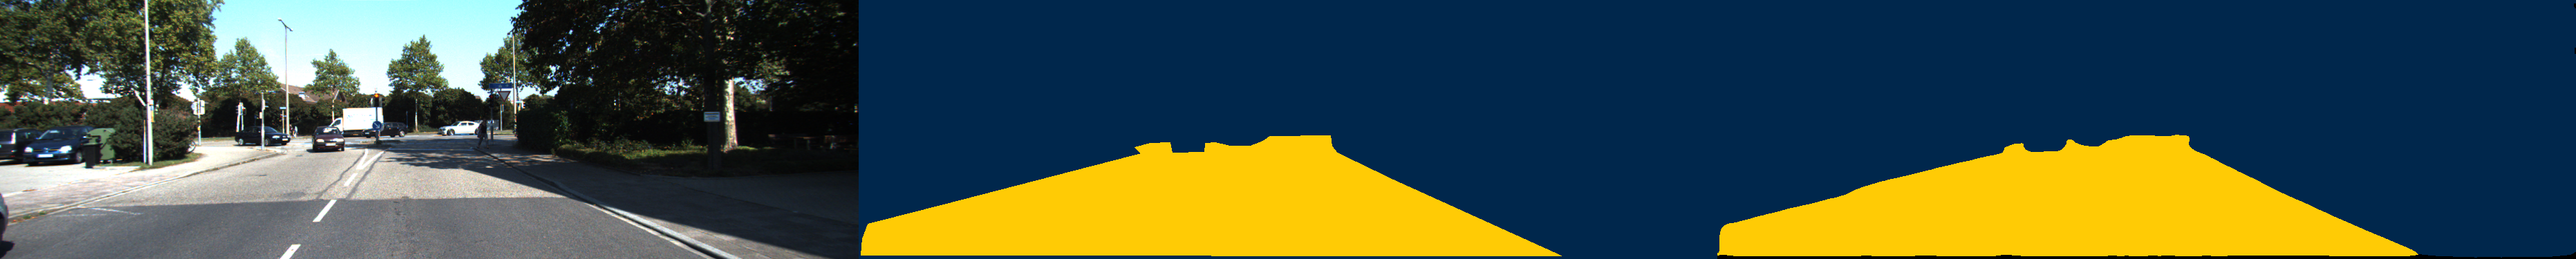
\includegraphics[width=0.9\linewidth]{images/rn100_b.png}
        \caption{ResNet50-Dilated with Pyramid Pooling Module}
    \end{subfigure}
    \caption{Selected images showing the results of the segmentation prediction. In each, the left most image is the image being segmented. The first segmentation is the ground truth, and the second segmentation is the prediction.}
    \label{fig:samples}
\end{figure*}

\section{Conclusions}
Looking at the images generated by each network, the HRNetV2 predictions very clearly more closely approximate the shape of the ground truth. I conclude this to be a result of the fact that HRNetV2 carries along the full resolution information to its predictions. It would be interesting to adapt some of the design elements of the PPM to the HRNet architecture in future work.

Through my experimentation, it is clear that even without purpose built networks specific to road segmentation, extremely high performance can be achieved. Furthermore, the most rapidly trained network only took two hours, and still performed quite well. The attention has largely shifted away from this problem and I believe this work shows just why - the performance is already more than good enough with the existing networks.

\section{Acknowledgements} I would like to thank Professor Andrew Owens and all of the course staff for a great semester and for providing me with the background knowledge required to complete this project.

{\small
\bibliographystyle{ieee_fullname}
\bibliography{egbib}
}

\end{document}
